% Created 2024-02-21 Wed 11:28
% Intended LaTeX compiler: pdflatex
\documentclass[presentation]{beamer}
\usepackage[utf8]{inputenc}
\usepackage[T1]{fontenc}
\usepackage{graphicx}
\usepackage{longtable}
\usepackage{wrapfig}
\usepackage{rotating}
\usepackage[normalem]{ulem}
\usepackage{amsmath}
\usepackage{amssymb}
\usepackage{capt-of}
\usepackage{hyperref}
\mode<beamer>{\usetheme{Madrid}}
\definecolor{SUred}{rgb}{0.59375, 0, 0.17969} % SU red (primary)
\definecolor{SUblue}{rgb}{0, 0.17578, 0.38281} % SU blue (secondary)
\setbeamercolor{palette primary}{bg=SUred,fg=white}
\setbeamercolor{palette secondary}{bg=SUblue,fg=white}
\setbeamercolor{palette tertiary}{bg=SUblue,fg=white}
\setbeamercolor{palette quaternary}{bg=SUblue,fg=white}
\setbeamercolor{structure}{fg=SUblue} % itemize, enumerate, etc
\setbeamercolor{section in toc}{fg=SUblue} % TOC sections
% Override palette coloring with secondary
\setbeamercolor{subsection in head/foot}{bg=SUblue,fg=white}
\setbeamercolor{date in head/foot}{bg=SUblue,fg=white}
\institute[SU]{Shenandoah University}
\titlegraphic{
\includegraphics[width=0.5\textwidth]{\string~/Documents/suLogo/suLogo.pdf}}
\usepackage{tikz}
\usetheme{default}
\author{Chase Mathison\thanks{cmathiso@su.edu}}
\date{22 February 2024}
\title{Trigonometric Integrals}
\hypersetup{
 pdfauthor={Chase Mathison},
 pdftitle={Trigonometric Integrals},
 pdfkeywords={},
 pdfsubject={},
 pdfcreator={Emacs 29.1 (Org mode 9.6.7)}, 
 pdflang={English}}
\begin{document}

\maketitle

\section{Announcements}
\label{sec:org4058208}
\begin{frame}[label={sec:orgf85f111}]{Announcements}
\begin{enumerate}
\item Don't forget about exam corrections.
\item Office hours 10am - 11am.
\end{enumerate}
\end{frame}

\section{Lecture}
\label{sec:orgeb79653}
\begin{frame}[label={sec:org7e4ef83}]{Today's mission}
Our goal today is to tackle three types of trigonometric integrals:
\begin{enumerate}
\item Integrals of the form \[\int\limits_{}^{} \cos^j \left( x \right)
   \sin^k \left( x \right)\,dx \] where \(k,j\) are nonnegative
integers (0,1,2,\ldots{}) and not both 0.
\item Integrals of the form \[\int\limits_{}^{} \sin(ax)\cos(bx)\,dx \]
for real numbers \(a\) and \(b\).
\item Integrals of the form \[\int\limits_{}^{} \tan^j \left( x \right)
   \sec^k \left( x \right)\,dx \] where \(k,j\) are nonnegative
integers.
\end{enumerate}
\end{frame}

\begin{frame}[label={sec:orgb9173a4}]{Today's mission}
Why do we need to cover these?

The main reason we need to cover these is that they will come up quite
frequently when we learn about trigonometric substitution tomorrow.
Let's begin by looking at 1.

Really the main idea behind most of what we do today lies in a handful
of trig identities and trig derivatives, but most importantly:
\begin{align*}
&\cos^2(x) + \sin^2(x) = 1,\,\frac{d}{dx}(\sin(x)) = \cos(x),\,\frac{d}{dx}(\cos(x)) = -\sin(x)\\
&1 + \tan^2 (x) = \sec^2(x),\,\frac{d}{dx}(\tan(x)) = \sec^2(x),\,\frac{d}{dx}(\sec(x)) = \sec(x)\tan(x)
\end{align*}
\end{frame}

\begin{frame}[label={sec:orga7a5c1f}]{Sines and Cosines}
There are 4 cases we could have when looking at the integral
\[
\int\limits_{}^{} \sin^k \left( x \right) \cos^j \left( x \right)\,dx
\]
We could have
\begin{enumerate}
\item \(k\) is even and \(j\) is even.  This is the annoying case.
\item \(k\) is even and \(j\) is odd.  This is a relatively easy case.
\item \(k\) is odd and \(j\) is even. This is handled almost exactly as
the second case.
\item \(k\) is odd and \(j\) is odd. This is also relatively simple and
handled in a similar way as 2 and 3.
\end{enumerate}

Let's look at specific examples, starting from the bottom, of each of these cases and then
generalize.
\end{frame}

\begin{frame}[label={sec:org967d243}]{\(k\) odd and \(j\) odd}
Find
\[
\int\limits_{}^{} \sin^3 \left( x \right)\cos^5 \left( x \right)\,dx
\]
\vspace{10in}
\end{frame}

\begin{frame}[label={sec:orgf238fac}]{\(k\) odd and \(j\) odd}
\end{frame}

\begin{frame}[label={sec:orgada7d29}]{\(k\) even and \(j\) odd}
Find
\[
\int\limits_{}^{} \sin^4 \left( x \right)\cos^5 \left( x \right)\,dx
\]
\vspace{10in}
\end{frame}

\begin{frame}[label={sec:org790e68a}]{\(k\) even and \(j\) odd}
\end{frame}

\begin{frame}[label={sec:org9119866}]{\(k\) odd and \(j\) even}
Find
\[
\int\limits_{}^{} \sin^5 \left( x \right)\cos^4 \left( x \right)\,dx
\]
\vspace{10in}
\end{frame}

\begin{frame}[label={sec:org33597bb}]{\(k\) odd and \(j\) even}
\end{frame}

\begin{frame}[label={sec:org14f1970}]{\(k\) even and \(j\) even (not both 0)}
Find
\[
\int\limits_{}^{}\sin^2 \left( x \right)\,dx \]
\vspace{10in}
\end{frame}

\begin{frame}[label={sec:orga2c3091}]{\(k\) even and \(j\) even (not both 0)}
\end{frame}

\begin{frame}[label={sec:org4cc009f}]{One more example}
Find
\[
\int\limits_{}^{} \sin^2 \left( x \right)\cos^2 \left( x \right)\,dx
\]
\vspace{10in}
\end{frame}

\begin{frame}[label={sec:org6db8377}]{In general}
In general, we can use this problem solving strategy when evaluating
integrals of this kind:
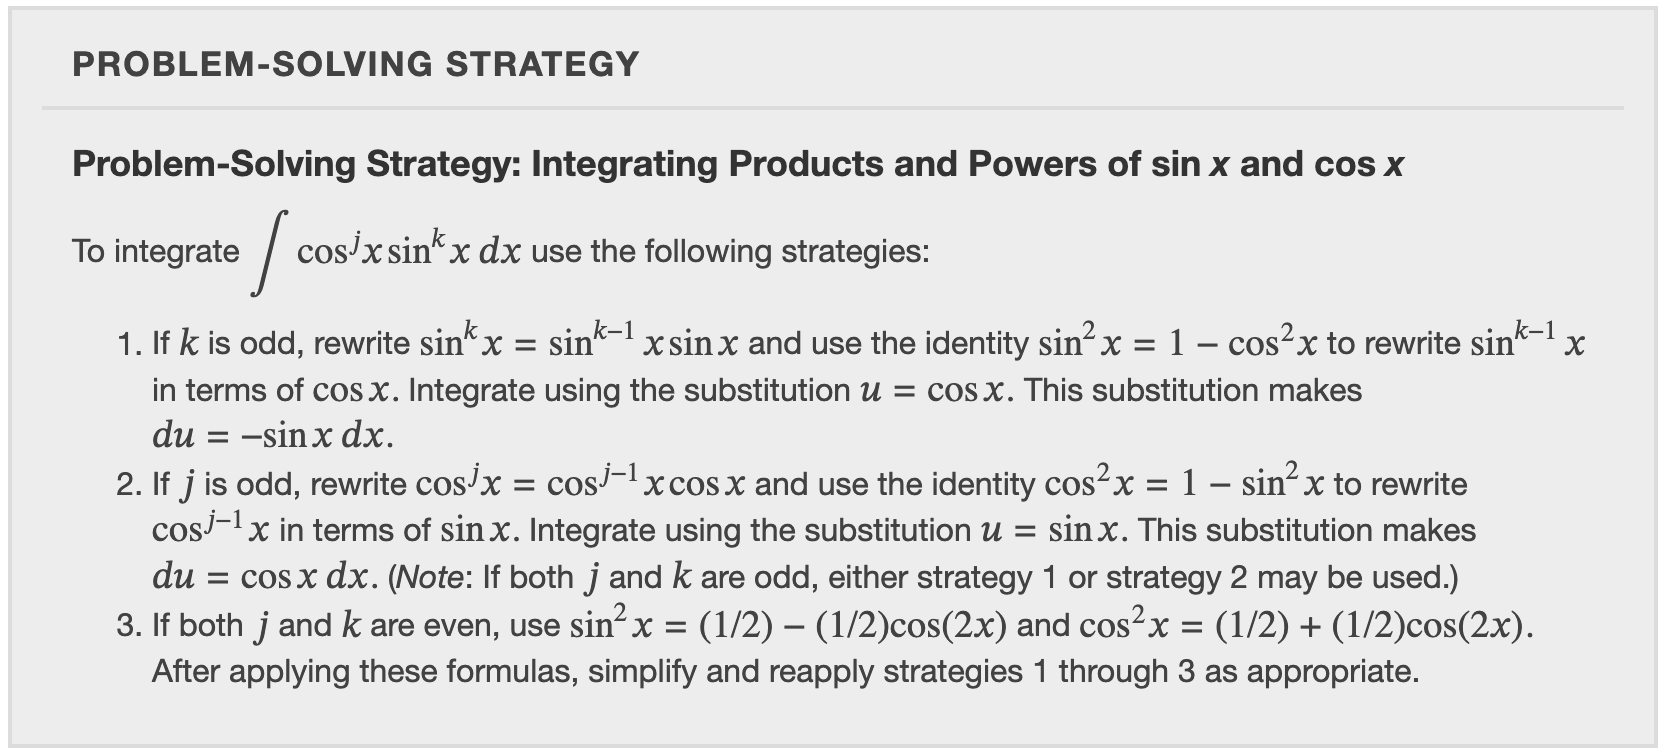
\includegraphics[width=\textwidth]{../img/day018-01.png}
\end{frame}

\begin{frame}[label={sec:orgf4f141b}]{Other sines and cosines}
We've seen how to integrate powers of sines and cosines, but what
about an integral of the form
\[
\int\limits_{}^{} \sin \left( 2x \right)\cos \left( 3x \right)\,dx? \]
We could do integration by parts and arrive back at the same integral
(my favorite type of integral), or we could take advantage of some
trig identities.
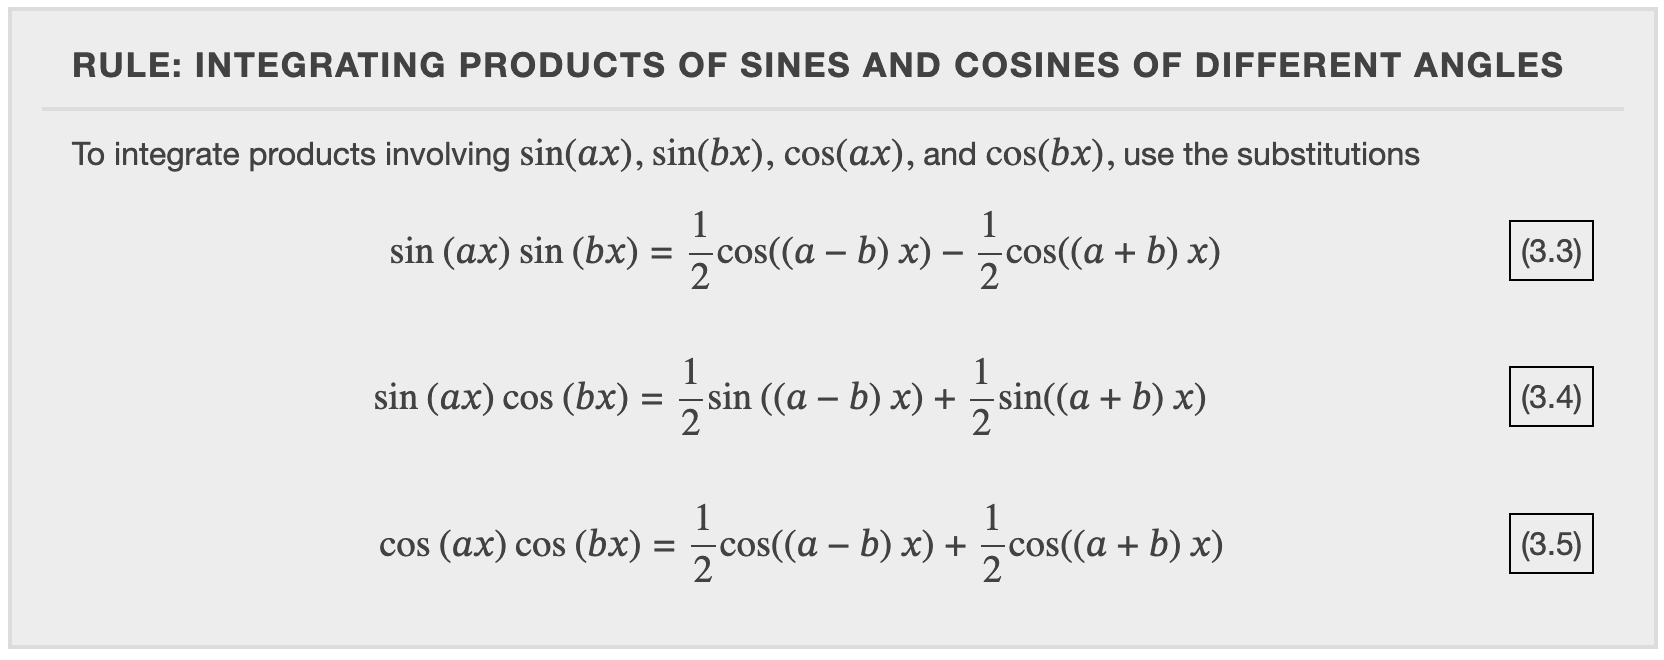
\includegraphics[width=\textwidth]{../img/day018-02.png}
\end{frame}

\begin{frame}[label={sec:orgc6cfe2e}]{Let's try it}
Evaluate
\[\int\limits_{}^{} \sin \left( 2x \right)\cos \left( 3x \right)\,dx
\]
using trig identities.
\vspace{10in}
\end{frame}
\end{document}